\chapter{Implementation}
\label{ch:implementation}
\label{sec:implementation}

This chapter summarizes the practical implementation used to instantiate and evaluate the theoretical models introduced in Chapter~\ref{ch:design_methodology}. The evaluation is organized around three complementary models. First, the end-to-end \gls{id} latency model is instantiated to generate bandwidth and desynchronization sensitivity plots. Second, the tolerance-based \gls{kid} protocol is evaluated by sweeping the physical tolerance radius $R$ and verifier length $n_{ver}$. For each $(R,\Delta)$ pair, the induced acceptance-set cardinality $K=|\mathcal{A}_R|$ follows the definition in Equation~\eqref{eq:kid_K_from_R}. Third, a time-correlated dynamic model is implemented in which \gls{kid} operates under random-walk drift, allowing accumulation effects such as sustained boundary breaches after missed corrections to be studied.

% Added for cross-reference from Chapter 5
\label{sec:implementation_design}

\section{Data Packet Structure Abstraction}
\label{sec:packet_structure}
While the analysis in Chapter~\ref{ch:design_methodology} models transmission cost in terms of $n_{ver}$ and $n_{data}$, practical deployments encapsulate these fields in a communication frame. Figure~\ref{fig:id_frame_structure} illustrates the abstract frame layout assumed in this thesis. In normal operation, the robot transmits only a compact verifier; when verification fails, the protocol falls back to transmitting the full state payload. The \gls{kid} protocol uses the same message structure as \gls{id}; it differs only in the receiver-side acceptance rule (set membership rather than strict equality).

In the latency model, the header, timestamp, and checksum/CRC are treated as fixed overheads and are omitted for clarity. If required, these can be incorporated by adding a constant number of bits to both the verifier-only and fallback frames.

\begin{figure}[!htbp]
    \centering
    \begin{tikzpicture}[
        field/.style={draw, minimum height=8mm, align=center, inner sep=2pt, font=\small, line width=0.4pt},
        rowlabel/.style={font=\bfseries\small},
    ]

        % Row 1: verifier-only
        \node[field, fill=black!8, minimum width=0.15\textwidth] (h1) {Header};
        \node[field, fill=blue!12, minimum width=0.40\textwidth, right=0pt of h1] (v1) {Verifier\\($n_{ver}$)};
        \node[field, fill=black!8, minimum width=0.25\textwidth, right=0pt of v1] (t1) {Timestamp};
        \node[field, fill=black!8, minimum width=0.15\textwidth, right=0pt of t1] (c1) {Checksum\\CRC};
        \draw[rounded corners=1pt, line width=0.6pt] (h1.north west) rectangle (c1.south east);
        \node[rowlabel, above=2mm of v1] {Verifier-only (\gls{id} / \gls{kid} normal tick)};

        % Row 2: fallback full payload
        \node[field, fill=black!8, minimum width=0.15\textwidth, below=10mm of h1] (h2) {Header};
        \node[field, fill=purple!12, minimum width=0.40\textwidth, right=0pt of h2] (p2) {State Payload\\($n_{data}$)};
        \node[field, fill=black!8, minimum width=0.25\textwidth, right=0pt of p2] (t2) {Timestamp};
        \node[field, fill=black!8, minimum width=0.15\textwidth, right=0pt of t2] (c2) {Checksum\\CRC};
        \draw[rounded corners=1pt, line width=0.6pt] (h2.north west) rectangle (c2.south east);
        \node[rowlabel, above=2mm of p2] {Fallback (full-state resynchronization)};
    \end{tikzpicture}
    \caption{Abstract \gls{id} message format used for modeling. The normal path transmits only a verifier, while the fallback path transmits the full state payload. Fixed overhead fields are shown for completeness but are not explicitly modeled in the latency equations.}
    \label{fig:id_frame_structure}
\end{figure}

\section{Software Architecture}
\label{sec:software_architecture}
A modular Python simulator supports rapid prototyping and evaluation of the proposed models.

Figure~\ref{fig:idsys_architecture} shows the high-level decomposition used throughout the Python experiments. The simulator is structured around three interchangeable components---Encoder, Channel/Dynamics, and Decoder/Decision. This separation allows swapping \gls{sha}-256 and \gls{rsid} encoders, switching between strict \gls{id} and tolerance-based \gls{kid} decision rules, and evaluating both i.i.d. and time-correlated models without entangling implementation details.

This modularity enables controlled comparisons: the experiment runner, channel models, and measurement pipeline remain fixed while only the encoder backend (\gls{sha}-256 vs. \gls{rsid}) and the receiver-side acceptance rule (\gls{id} vs. \gls{kid}) are varied.

The interface between Encoder and Channel is a transmitted packet/frame. In normal operation this contains only a verifier tag; on fallback it contains the full state payload. This matches the message abstraction in Figure~\ref{fig:id_frame_structure}.

\begin{figure}[!htbp]
    \centering
    \begin{tikzpicture}[
        font=\small,
        node distance=10mm and 6mm,
        box/.style={draw, rounded corners=2pt, align=center, inner sep=6pt, text width=0.255\textwidth},
        impl/.style={draw, rounded corners=2pt, align=left, inner sep=5pt, fill=black!4, text width=0.255\textwidth},
        arrow/.style={-Latex, line width=0.6pt},
        group/.style={draw, rounded corners=2pt, inner sep=6pt}
    ]
        % Top-level pipeline
        \node[box, fill=black!6] (sim) {Experiment Runner\\(sweep / Monte Carlo)};
        \node[box, fill=blue!8, below=10mm of sim] (enc) {Encoder\\$\mathrm{Enc}(\cdot)$};
        \node[box, fill=orange!10, right=6mm of enc] (chan) {Channel / Dynamics\\$\mathcal{C}(\cdot)$};
        \node[box, fill=green!10, right=6mm of chan] (dec) {Decoder / Decision\\$\mathrm{Dec}(\cdot)$};

        \draw[arrow] (sim) -- (enc);
        \draw[arrow] (enc) -- (chan);
        \draw[arrow] (chan) -- (dec);

        % Implementations
        \node[impl, below=8mm of enc] (encimpl) {\textbf{Implementations:}\\- \gls{sha}-256 (truncated)\\- \gls{rsid} (algebraic)};
        \node[impl, below=8mm of chan] (chanimpl) {\textbf{Models:}\\- i.i.d. desync $p_{desync}$\\- time-correlated drift (random walk)};
        \node[impl, below=8mm of dec] (decimpl) {\textbf{Rules:}\\- \gls{id}: strict equality\\- \gls{kid}: accept within tolerance $|e|\le R$};

        \draw[arrow] (enc) -- (encimpl);
        \draw[arrow] (chan) -- (chanimpl);
        \draw[arrow] (dec) -- (decimpl);
    \end{tikzpicture}
    \caption{High-level simulator architecture used in the Python experiments. Encoder, Channel/Dynamics, and Decoder are decoupled so that coding schemes (\gls{sha}-256 vs. \gls{rsid}), acceptance rules (\gls{id} vs. \gls{kid}), and stochastic models (i.i.d. vs. time-correlated drift) can be varied independently.}
    \label{fig:idsys_architecture}
\end{figure}


\section[K-ID Simulation Setup and Implementation]{\glsentryshort{kid} Simulation Setup and Implementation}
\label{sec:kid_setup}

This section outlines the simulation environment used to instantiate the \gls{kid} framework from Chapter~\ref{ch:design_methodology}. The objective is to quantify the trade-off between the physical tolerance radius $R$ and safety risks under constrained edge-link conditions. In the simulator, $R$ is the physical threshold in the state space, while $K$ denotes the induced acceptance-set size $K=|\mathcal{A}_R|$ used in the collision analysis (Equation~\eqref{eq:pmiss_law}).

\subsection{Error Models and State Generation}
\label{subsec:error_models_impl}

The simulation models the robot's state as a continuous random variable constrained to a physical domain of 0 to 100. To evaluate the impact of error distribution shapes, two contrasting noise models are instantiated while controlling for their noise energy.

The baseline Gaussian model is centered at the domain midpoint with a standard deviation of $\sigma=16.0$. This parameter choice maximizes utilization of the physical state space without violating boundaries, ensuring that the simulation includes rare but safety-relevant tail events. For the comparative Uniform model, a variance-matching constraint is applied to isolate the effect of bounded support. For a symmetric uniform distribution on $[-a,a]$, $\mathrm{Var}=a^2/3$; equating $a^2/3=\sigma^2$ yields $a=\sqrt{3}\,\sigma\approx 27.71$.

This half-width defines a \emph{safe-harbor} threshold: choosing $R\ge a$ guarantees $|e|\le R$ for all samples under the Uniform model and therefore eliminates tolerance violations by construction.

\begin{figure}[htbp]
    \centering
    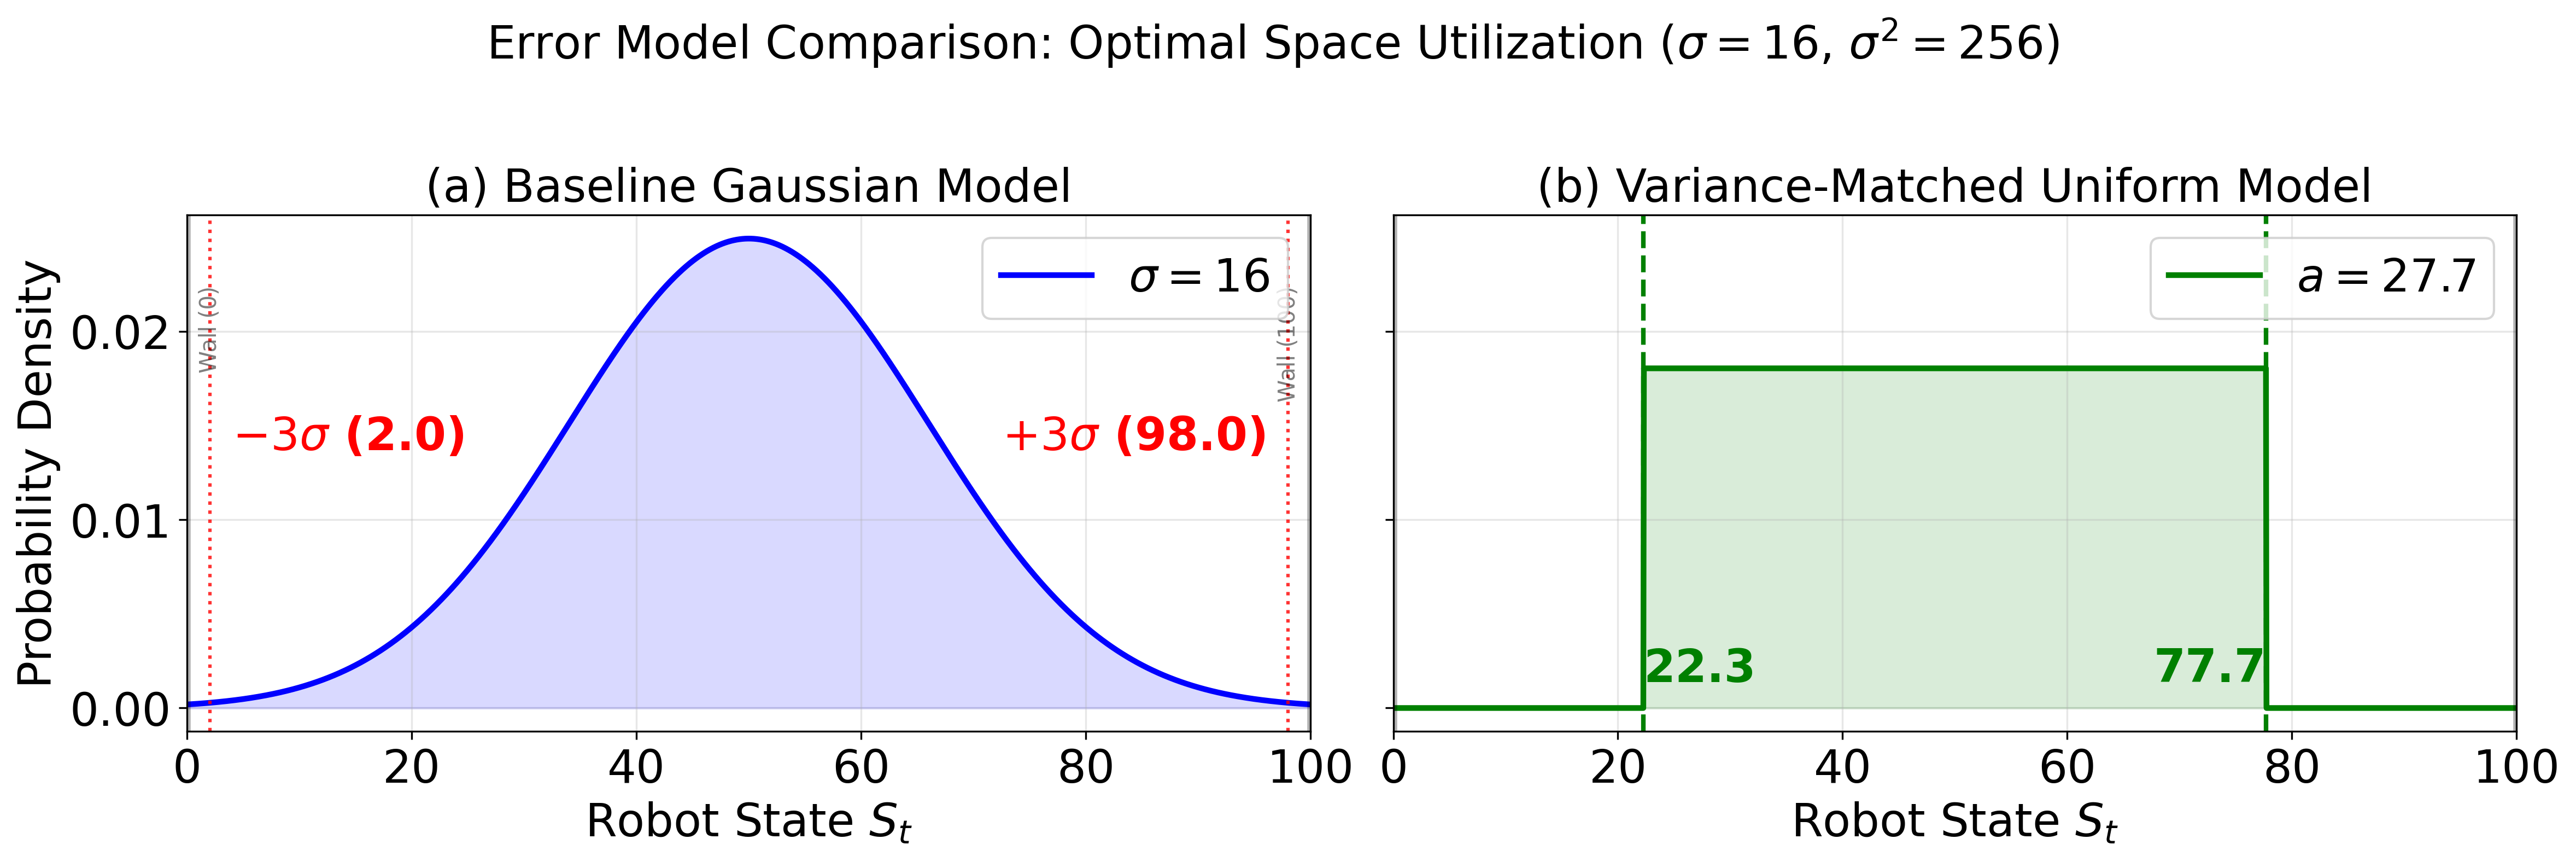
\includegraphics[width=1.0\textwidth]{figures/error_models_sigma16.png}
    \caption{Visual comparison of the variance-matched error models configured with $\sigma=16$. The Gaussian baseline (a) maximizes physical space utilization within the domain bounds $[2, 98]$, preventing truncation artifacts while maintaining high noise energy. The Uniform model (b) illustrates the safe-harbor threshold: the selected tolerance radius of 30 exceeds the noise support, guaranteeing zero tolerance-violation risk under the Uniform model, whereas the Gaussian model retains residual tail risks outside the tolerance zone.}
    \label{fig:error_models}
\end{figure}

\subsection{Computational Scalability and Latency Model}
\label{subsec:scalability_model}

A sensitivity analysis quantifies the computational scalability of the \gls{kid} decoder by sweeping the quantization resolution $\Delta$ from 1.0 down to 0.01. The total decoder latency is modeled linearly as the product of the acceptance-set cardinality $K$ and the unit verification overhead; since $K$ grows approximately as $K\propto R/\Delta$ (Equation~\eqref{eq:kid_K_from_R}), finer quantization increases computation even when $R$ is fixed.

The results of this sensitivity sweep reveal a scalability bottleneck governed by the resolution. As the quantization becomes finer, the computational cost grows hyperbolically. For large-tolerance configurations, high-precision settings drive the decoder latency well beyond typical control budgets. Relaxing the resolution to 0.1 reduces the worst-case latency to approximately 1.3 ms, balancing precision with feasibility. Consequently, this operating point is selected as the fixed resolution for subsequent experiments.

\begin{figure}[H]
    \centering
    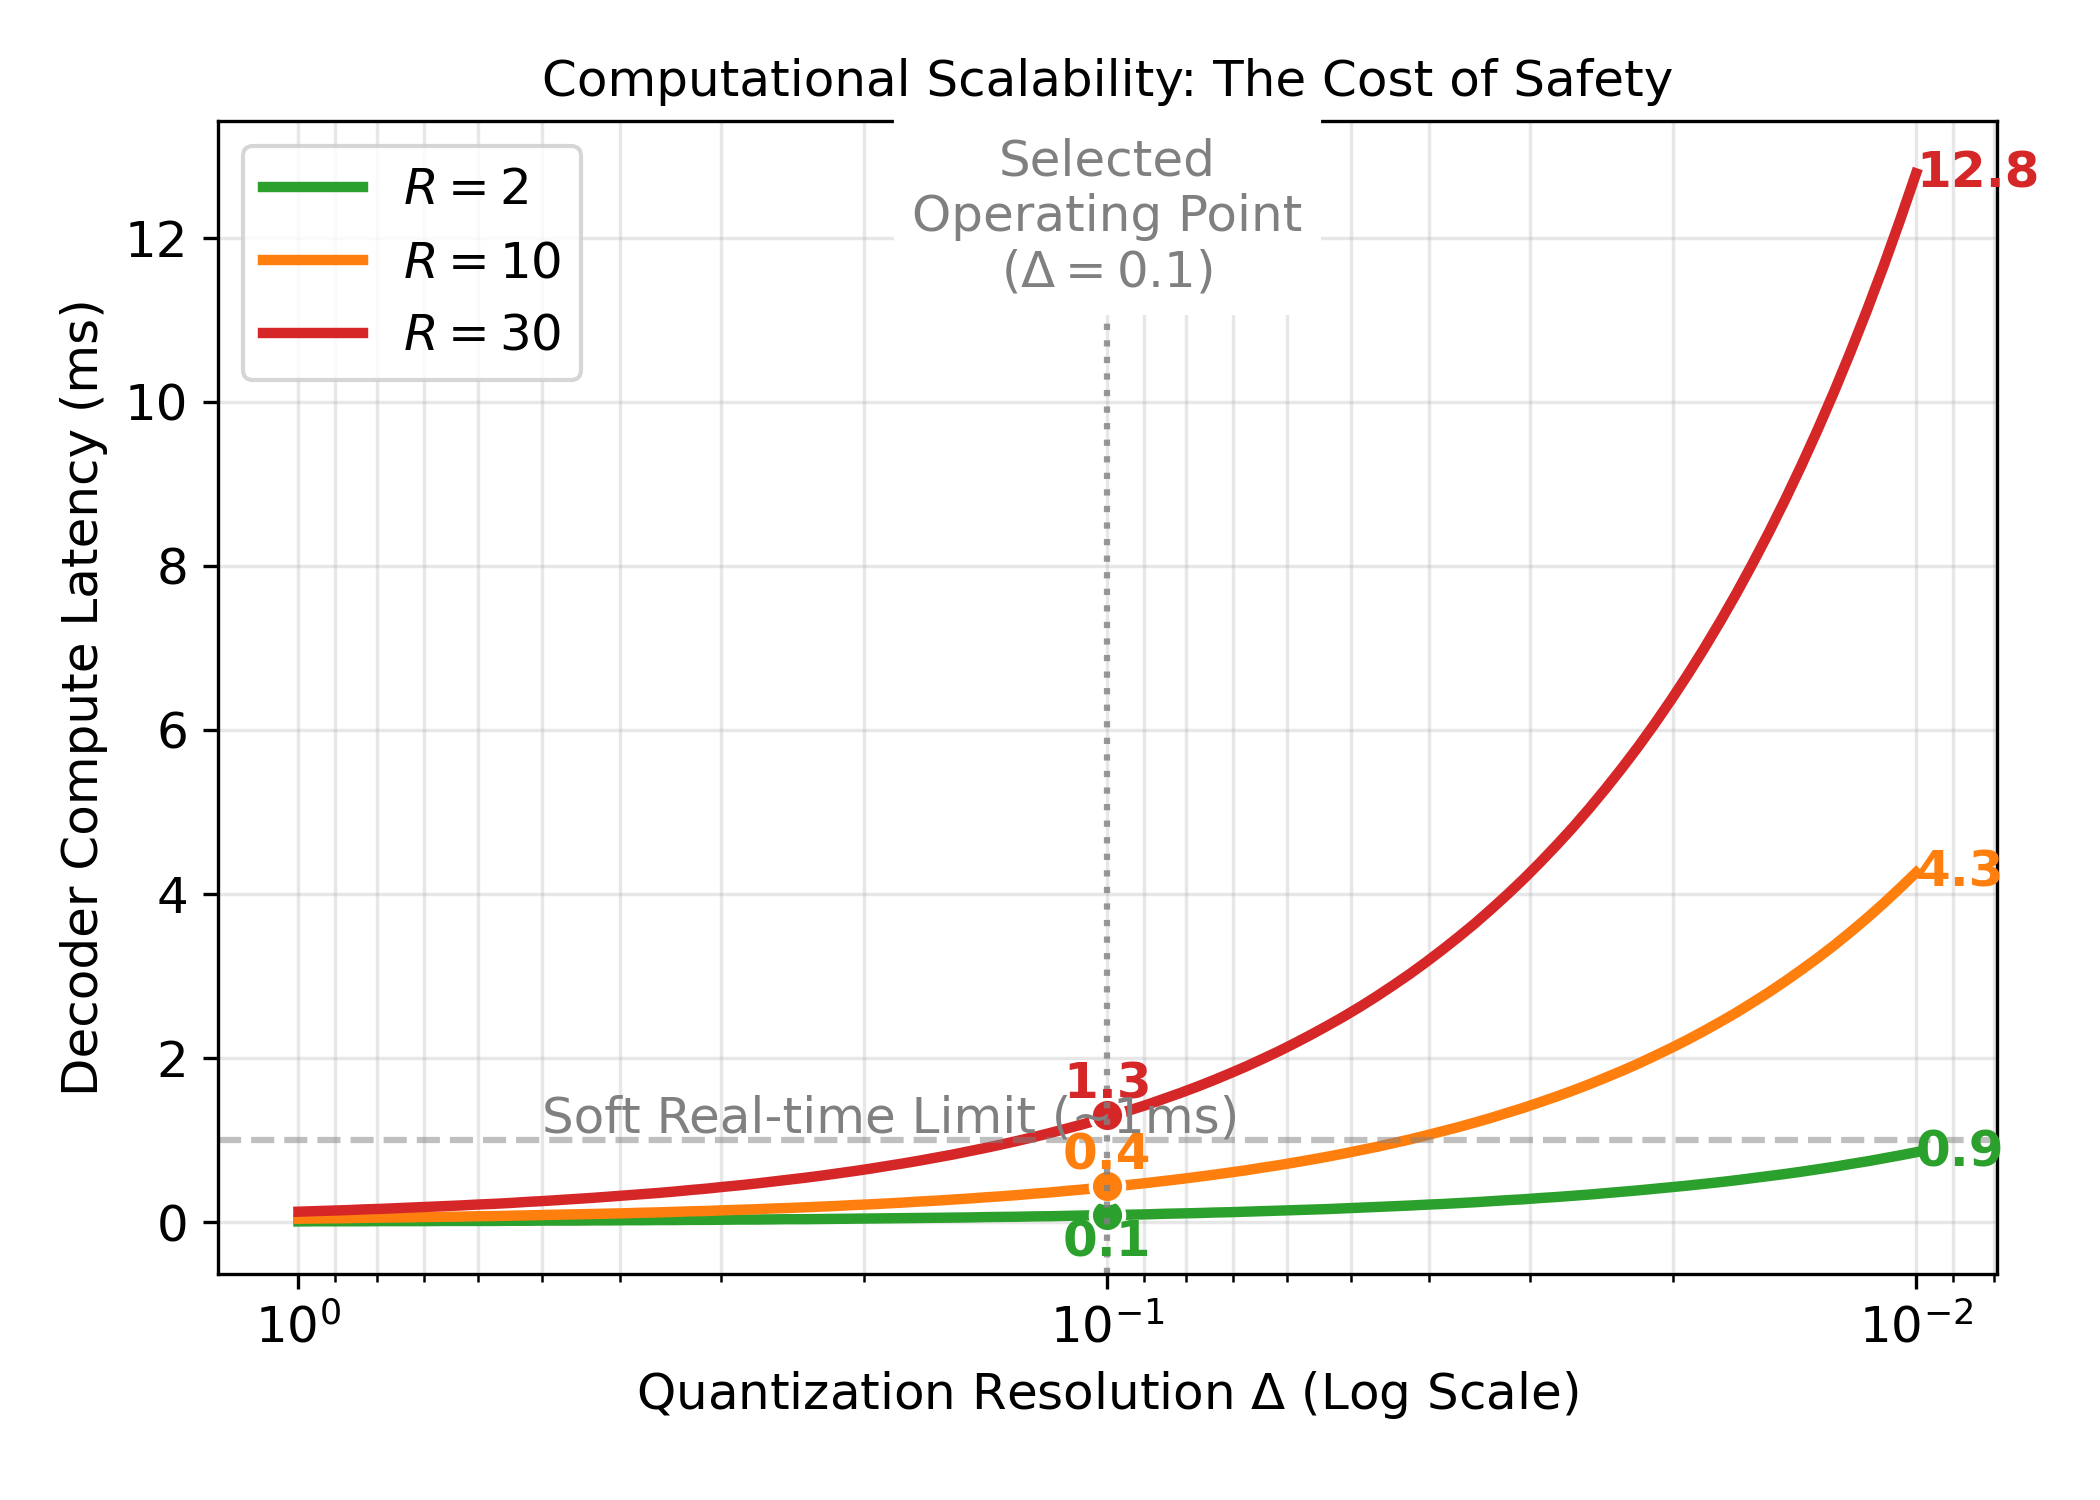
\includegraphics[width=0.72\linewidth,height=0.32\textheight,keepaspectratio]{figures/decoder_cost_multiline_annotated.png}
    \caption{Computational scalability analysis showing decoder latency as a function of quantization resolution $\Delta$. The red curve represents the safe-harbor configuration ($R=30$). At the high-precision limit ($\Delta=0.01$), latency reaches a prohibitive 12.8 ms. However, at the selected operating point ($\Delta=0.1$, indicated by the vertical dotted line), the latency drops to approximately 1.3 ms, balancing maximum physical coverage with real-time computational feasibility.}
    \label{fig:decoder_scalability}
\end{figure}

\subsection{System Configuration and Visualization}
\label{subsec:param_config}

The primary simulation assumes a payload of 4001 bits transmitted over a 1 Mbps link. The evaluation framework employs the physical tolerance radius $R$ as the primary independent variable to maintain a direct mapping to robotic safety requirements. The sweep uses $R\in\{2,5,10,20,30\}$. The largest value is motivated by the Uniform half-width derived above ($a\approx 27.71$), which provides a boundary condition where tolerance violations vanish under bounded noise.

To analyze the trade-off space, a dual visualization strategy is employed. Raw simulation results are mapped onto a grid defined by verifier length and physical tolerance to display speedup factors and risk probabilities. These points are subsequently projected onto a risk-vs-speedup scatter plot to extract the Pareto frontier.

\section{Dynamic Evaluation Framework: The Random Walk Model}
\label{sec:dynamic_evaluation}

To evaluate \gls{kid} under continuous operation, a discrete-time simulation framework is used comprising a stochastic robot agent, a bandwidth-constrained channel, and a \gls{dt} receiver. Unlike the static sweeps in Section~\ref{sec:kid_setup}, this dynamic evaluation models time-correlated accumulation of drift, allowing safety risks that only emerge over extended trajectories to be quantified.

\subsection{Dynamic Protocol Logic}
The robot's state evolution is modeled as a diffusive process, specifically a Gaussian random walk defined by $S_t = S_{t-1} + \delta_t$, where the increment follows a normal distribution with a unit step deviation. This standardized diffusion ensures the variance of the uncorrected state grows linearly with time, providing a reproducible challenge for the synchronization protocol.

The \gls{kid} protocol operates as a guardrail mechanism on this state evolution. At each time tick, the absolute deviation between the true state and the \gls{dt} estimate is evaluated. If the deviation remains within the tolerance radius ($|e|\le R$), the protocol remains silent; if $|e|>R$, a verification event is triggered.

For long-horizon simulation, the encoder backend is abstracted as a probabilistic verification model grounded in the Chapter~2 reliability law (Equation~\eqref{eq:pmiss_law}). Specifically, the verification outcome at a check event is implemented as a Bernoulli trial with miss probability $p_{miss}\approx K/2^{n_{ver}}$, where $K=|\mathcal{A}_R|$ is induced by $(R,\Delta)$ (Equation~\eqref{eq:kid_K_from_R}). This abstraction preserves the theoretically derived dependence on $(K,n_{ver})$ while decoupling the experiment logic from implementation-specific hashing costs.

\subsection{Experimental Strategy}
The evaluation strategy consists of two complementary phases. First, a qualitative stress test is used to induce observable failure modes. By intentionally reducing $n_{ver}$, the collision probability increases, which amplifies otherwise rare long-tail events and makes sustained boundary breaches observable within a manageable simulation window.

Second, a quantitative parameter sweep systematically varies the tolerance radius and verifier length while fixing the drift dynamics. This grid search decouples the masking effect of physical tolerance from the collision risk of the verification step, providing the statistical basis for the trade-off analysis.

\subsection{Metrics for Dynamic Safety}
To quantify the trade-off between efficiency and risk, three primary metrics are defined. The Successive Recovery Interval (\gls{sri}) measures the number of ticks between two consecutive recovery-triggered check events (i.e., transmission attempts triggered by $|E_t|>R$). In the simulator, this quantity is equivalent to the inter-check interval (\gls{ift}); a larger \gls{sri} indicates higher masking efficiency and reduced channel contention.

Safety is assessed via two complementary metrics. The Breach Duration counts the number of consecutive ticks during which the system remains in an unsafe state due to hash collisions, measuring the temporal persistence of safety violations. Finally, the Maximum Drift metric records the peak absolute error reached during a simulation run. Unlike Breach Duration, this quantifies the worst-case physical magnitude of the error, serving as a proxy for potential physical damage in control scenarios.

